\section{Conclusion and Outlook}
\label{sec:sum}

In this work, we proposed a new method to generate quantum field configurations using diffusion models, popular in the ML community. We highlighted the connection with stochastic quantization (SQ), an approach to quantize field theories based on a stochastic process in a fictitious time direction. In SQ the drift term in the stochastic process is known, as it is derived from the probability distribution one wants to sample from, which is determined by the quantum theory under consideration. In DMs the drift term is not known but is learned from data in a forward stochastic process. After estimating the drift term, the trained DM is run in the opposite direction and independent configurations are created from noise, the ``denoising'' process. This latter part is akin to the dynamics in SQ, albeit with a learned and time-dependent drift term. {In Figure~\ref{fig:flow-chart}, we summarize the relation between stochastic quantisation and diffusion models schematically.}

%%%%%%%%%%%%%%%%%%%%%%%%%%%%%%%%%%%%%%%%%%%%%%%%%%%%%%%%%%%%%%%%%%%%%%%%%%%%%%%%%%%%%%%%%%%%%%%%%%%%%%%%%%%%%%%%%%
\begin{figure}[hbtp!]
    \centering
    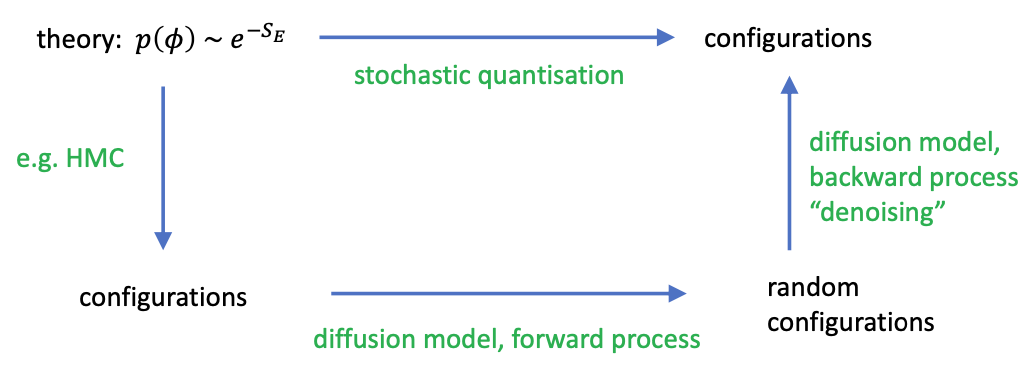
\includegraphics[width = 0.7 \textwidth]{images/flow-chart.png}
    \caption{Schematic overview of the relation between stochastic quantisation and diffusion models in the case of lattice field theory. }
    \label{fig:flow-chart}
\end{figure}
%%%%%%%%%%%%%%%%%%%%%%%%%%%%%%%%%%%%%%%%%%%%%%%%%%%%%%%%%%%%%%%%%%%%%%%%%%%%%%%%%%%%%%%%%%%%%%%%%%%%%%%%%%%%%%%%%%

We have demonstrated the approach in a simple toy model and in a two-dimensional scalar field theory with a $\phi^4$ interaction, both in the symmetric and in the broken phase. We have shown that the DM can serve as a global sampler to assist methods based on the Monte Carlo principle. We note that one can include an accept-reject step at the end of each trajectory. We have found in our numerical results that the well-trained DM can successfully reproduce configurations in both phases and that autocorrelation times are reduced along a Markov chain. This improvement in sampling efficiency can be beneficial for studying lattice field theories and should be analyzed further. 

There are various directions to explore in the future. The forward (``smoothening") and backward (``denoising") processes are reminiscent of (inverse) renormalization group transformations and it would be interesting to make this precise.   
Because the action can be estimated relatively accurately, it is feasible to train a DM without preparing a training data-set, which needs to be investigated.
The connection between DMs and SQ offers new perspectives. It is well known how to implement SQ for non-abelian gauge theories; hence it should be possible to formulate DMs for the non-abelian case. An intriguing direction is the following: imagine one has generated a set of configurations for a quantum field theory with fermions, such as QCD or the Schwinger model. Since the fermions are ``integrated out'', the configurations are given in terms of the gauge fields only. By using these configurations as the starting point of a DM, one can learn an effective stochastic process which incorporates the effect of the fermions implicitly. This may be used to create additional configurations in a numerically ``cheap" manner. An accept-reject step based on the underlying theory can be included, which would require the evaluation of the fermion determinant. Finally SQ can also be used for theories with a sign or complex action problem, and hence a non-positive definite distribution. This is commonly known as complex Langevin (CL) dynamics. It is known that CL may become less reliable along long trajectories in the stochastic process. Combining CL with DMs, one may consider fairly short trajectories, but subsequently use the resulting configurations to train the DM to generate additional configurations to increase statistics. 

